\documentclass[%
aip,
cp,  % Conference Proceedings
amsmath,amssymb,
reprint,%
]{revtex4-2}

\usepackage{graphicx}% Include figure files
\usepackage{dcolumn}% Align table columns on decimal point
\usepackage{bm}% bold math
\usepackage[utf8]{inputenc}
\usepackage[T1]{fontenc}
\usepackage{mathptmx}
\usepackage{booktabs}
\usepackage{tabularx}
\usepackage{float}
\usepackage[caption=false,font=footnotesize]{subfig}
\usepackage{cleveref}

\begin{document}
	
	\title{A Hybrid ACO-Reinforcement Learning Framework for Task Assignment}
	
	\author{Sampath Kumar}
	\email{sz4961@srmist.edu.in}
	\affiliation{Department of Computer Science Engineering, SRM Institute of Science and Technology, Chennai, India}
	
	\author{Dr.Krishnaraj N}
	\email{krishnan2@srmist.edu.in}
	\affiliation{Department of Networking And Communications, SRM Institute of Science and Technology, Chennai, India}
	
	\date{\today}
	
	\begin{abstract}
		This paper presents a new approach on combining Ant Colony Optimization (ACO)
		with Reinforcement Learning (RL) techniques employing Q-learning and SARSA,
		to organize and allocate tasks in complex work environments. This approach addresses
		issues with order of task execution, diverse employee skills, employee availability,
		and fair workload distribution. ACO creates an initial task sequence considering
		dependencies and deadlines. Using the ACO determined task sequence, RL agents
		determine the initial assignments by basing their decisions depending on skill
		fit, workload distribution along with deadlines. This approach uses a multi objective
		hyperparameter tuning with Optuna library to balance high rate of task assignment
		with workload distribution."Refinement RL" component provides final passthrough
		by balancing the workload across the skills to ensure employees are not overloaded.
		Experiments reveal that in task assignment rate and workload distribution, the
		ACO-RL combination performs better than simple greedy approach. This study
		adds to ongoing research on scheduling and task assignment optimization
		problems in complex industrial setups.
	\end{abstract}
	
	\keywords{Reinforcement learning, Task scheduling, Resource allocation, Ant colony optimization, Manufacturing systems, Skill matching, Workload balancing}
	
	\maketitle
	
	\section{\label{sec:intro}Introduction}
	Task assignment in industrial settings, for both people or machines, is a hard
	problem to solve while achieving smooth operations and strong employee management.
	This because of the requirement of optimal task assignments taking account of the limit of employees, hours skills and  efficiency. As Zhang et al. (2022) have shown, old ways of scheduling tasks according to fixed rules and simple ideas do not work in fast changing work settings, for example, heuristic based methods cannot effectively deal with dynamic job-shop environments with uncertainties such as unexpected machine failures and rapidly changing market demands\cite{zhang2022, li2024}.
	
	\subsection{\label{subsec:challenges}Challenges Across Sectors}
	This problem compounds even more in different sectors that rely heavily on
	task planning. In factories good scheduling and assignment can stop production
	delays or extra costs. Hospitals need schedules that meet patient needs while
	matching available staff and laws. Tech teams require loose schedules to handle
	sudden project changes. Call centres must keep service steady while facing
	varying demand.
	
	\subsection{\label{subsec:remote}Impact of Remote Work}
	To make matters complicated the increase in remote and hybrid work has complicated scheduling and task assignments.Remote work offers enhanced flexibility and autonomy, allowing employees to manage their work schedules and surroundings, thereby fostering a better work-life balance \cite{wang2023}. Companies must take in to account: time zones, the nature of employee availability, sharing of employee between projects, their skills and frequent attrition. Old ways of scheduling and assignments based on "first come first assign" kind of greedy methodologies do not really fit well with the fast moving nature of modern businesses.
	
	
	
	\subsection{\label{subsec:hybrid}Proposed Hybrid Approach}
	This study proposes a framework (Fig.~\ref{fig:flow}) for the complex task
	assignment problem in an industrial setting with task dependencies and
	employee availability constraints, combining Reinforcement Learning and Ant Colony
	Optimization. First, we begin with task sequencing by ACO, which determines an
	optimal task sequence that satisfies task dependencies, due date, and priority
	restrictions. Then, we devise an initial employee assignment using
	Reinforcement Learning—specifically, Q-learning and SARSA (for comparison).
	Reward shaping guides these initial assignments by ensuring skills match, deadlines
	are met, work is balanced, and resources are used efficiently. Finally, a custom
	component named ``RefinementRL'' takes these initial assignments and optimizes
	them using a state representation that captures the workload, assignment, and unassigned
	tasks. Ultimately, the goal is to maximize a skill-level-based workload allocation
	and task assignment rate.
	
	\begin{figure}[!hb]
		\centering
		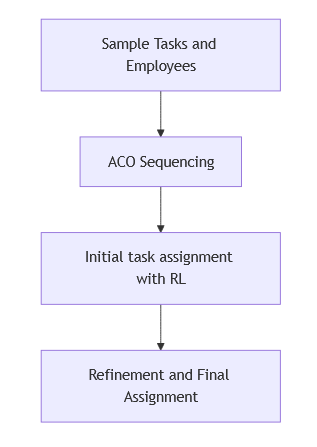
\includegraphics[width=0.3\linewidth]{figures/Initial_flow}
		\caption{\label{fig:flow}Proposed methodology}
	\end{figure}
	
	\subsection{\label{subsec:significance}Significance}
	Significance of this study comes from the integration of Reinforcement Learning
	with Ant Colony Optimization in task assignment optimization problem, which
	approaches the focus of critical workforce management and resource allocation
	issue. It demonstrates how meta heuristic algorithms can improve the current reinforcement
	learning approaches in complex scheduling environment.
	
	The general applicability of the framework is largely important due to its wide
	use in various industries, for example manufacturing to software development
	where it is important for resource constrained scheduling and skilled task
	assignment. Additionally, the framework allows RL component to continuously
	learn from experience and the ACO component to manage task sequencing in an
	efficient manner which is a major progress compared to traditional static
	methods of assignments. The practical solutions provided in this paper to industry-wide
	resource optimization problems contribute to both the academic literature on hybrid
	AI systems.
	
	\section{\label{sec:lit}Literature Survey}
	Reinforcement Learning (RL) has developed into a promising technique for dynamic
	environment workload optimization and task scheduling during the past years.
	Traditional heuristics and rule-based methods lose their value as scheduling
	problems become more advanced so adaptive RL-based approaches step in to
	replace them. The paper examines previous studies which examine reinforcement learning
	alongside associated optimization approaches for workload distribution and task
	distribution and scheduling in uncertain environments.
	
	Dynamic scheduling in job shops is difficult due to unexpected events. Ren and Liu~\cite{li2024} have developed a method that combines MachineRank assessments of machine utilization (including incoming jobs for processing at machines and outgoing ones) with D3QN to dynamically adjust schedules to improve the maximum completion times and increase on-time job completions.
	
	In similar scenario, Zhang et al.~\cite{zhang2022} have used Proximal Policy Optimization (PPO), a form of Deep Reinforcement Learning, to focus their efforts. Their approach adapted quickly to actual failures when tested with them, whereas conventional techniques lagged behind.
	
	The research by Infantes et al.~\cite{infantes2024} explores Deep
	Reinforcement Learning (DRL) solutions for Job-Shop Scheduling Problems (JSSP)
	under uncertain conditions. GNNs enable the enhancement of DRL model generalization
	and scalability according to their research. DRL proves successful for
	managing unpredictable task duration fluctuations and outperforms conventional
	deterministic methods according to their examination.
	
	Burdett and Kozan~\cite{burdett2004} study scheduling with limited resources
	and renewable resource assignment. The authors applied heuristic-based mathematical
	models for workforce allocation to develop constraint models that may be integrated
	into RL-based scheduling systems.
	
	The paper by Zhong~\cite{zhong2024} examines how Q-learning performs against SARSA
	reinforcement learning methods for task assignment. SARSA delivers stable
	solutions through its on-policy approach yet Q-learning achieves higher but
	riskier rewards by using its off-policy exploration method. Experts need these
	understandings to develop RL models which effectively manage exploration against
	exploitation for actual scheduling situations.
	
	Ben Noureddine et al.~\cite{noureddine2017} introduces multi agent
	reinforcement learning through Deep Q-learning to handle distributed task
	allocation. Through proposed agent teamwork operators gain better resource usage
	and less conflict during scheduling. The method proves beneficial for
	distributed systems which lack access to global information.
	
	The research by Joo et al.~\cite{joo2022} applies reinforcement learning methods
	to human-machine manufacturing systems. The research team developed a DRL
	model to handle human fatigue and skill abilities when performing dynamic task
	assignments. The research shows how human performance limitations integrated into
	RL-based scheduling systems produces more efficient operations and lowers worker
	exhaustion levels.
	
	The research by Wibisono et al.~\cite{wibisono2016} introduces a human-centered
	strategy for allocating resources during business process execution. The research
	supports RL-based scheduling by recommending real-time worker preference and availability
	assessment during scheduling operations.
	
	Dastmalchian and Blyton~\cite{dastmalchian2001} analyze how modern work patterns
	require adaptable scheduling systems. The research demonstrates that workforce
	adaptability needs to become part of all future task allocation models.
	
	Dorigo and Stützle~\cite{dorigo2016} deliver an extensive review of Ant Colony
	Optimization (ACO) and its scheduling problem applications. The bio-inspired optimization
	method ACO demonstrates great effectiveness when solving hard-to-tackle optimization
	problems. The review presents hybridization methods which use reinforcement
	learning to enhance task allocation efficiency.
	
	Sreyas Ramesh \textit{et al.}~\cite{turn0file0} investigate the application of Q-learning, SARSA, and deep Q-networks (DQN) for microgrid energy management. The authors compare these reinforcement learning methods in a simulated microgrid environment and demonstrate that while DQN achieves superior performance, traditional techniques like Q-learning and SARSA offer advantages in terms of computational simplicity and ease of implementation.
	
	Sivamayil \textit{et al.}~\cite{turn0file1} provide a systematic study of reinforcement learning applications across diverse domains, including energy management, robotics, and finance. Their review categorizes RL methodologies and highlights that the choice between value-based and policy-based approaches, such as Q-learning and SARSA, should be guided by the specific dynamics and requirements of the application at hand.
	
	In \cite{Corazza2015}, the authors address a stochastic control problem by comparing two reinforcement learning algorithms: Q-Learning and SARSA. The study focuses on developing an intelligent trading system that operates under the Adaptive Market Hypothesis. Both algorithms are tested on simulated and real stock price time series, with the research emphasizing the trade-offs between off-policy and on-policy learning methods in adapting to non-stationary market conditions. Their results demonstrate that while both methods are capable of adapting trading strategies based on real-time feedback, nuances in learning rates and exploration strategies critically impact overall performance.
	
	For this study we use Optuna by T. Akiba et al \cite{Akiba2019Optuna}. Optuna is a next generation hyperparameter optimization framework which provides a define-by-run API to build complex search spaces, and easily tune hyperparameters in an interactive as well as a distributed manner, compared to the static static methods.
	
	We also use Upper Confidence Bound (UCB) strategy. In their study \cite{Wang2023TaskScheduling}, Wang et al propose a new reinforcement learning (RL) framework, Q-learning based Multi-Task Scheduling Framework (QMTSF), for cloud task scheduling. Their approach consists of a two-stage process where tasks are first dynamically allocated to appropriate servers and then scheduled to virtual machines (VMs) using an enhanced Q-learning algorithm that incorporates the Upper Confidence Bound (UCB) strategy.By leveraging the UCB strategy—which balances exploration (trying new actions) and exploitation (using known rewards) and is more efficient than traditional methods such as the epsilon-greedy approach—the algorithm achieves faster convergence. Consequently, QMTSF reduces the overall makespan (i.e., the total time to complete all tasks) and average task processing time, as well as enhances energy efficiency and CPU utilization in the dynamic and heterogeneous cloud computing environment.
	
	Sutton and Barto’s \textit{Reinforcement Learning: An Introduction}\cite{SuttonBarto1998} is a go-to guide for anyone curious about Reinforcement Learning. This scholarly work elaborates algorithms like Q learning and policy iteration in detailed manner.
	
	
	\section{\label{sec:problem}Problem Formulation}
	
	In modern manufacturing and service environments, the allocation of tasks to a
	diverse workforce poses a complex, multi-objective challenge. The aim is to
	maximize the number of tasks successfully assigned while ensuring that
	deadlines are met, workloads are balanced, and employees' skills are
	effectively utilized. To address this, our methodology decomposes the problem
	into distinct but interrelated phases, integrating bio-inspired optimization,
	adaptive learning, and post-assignment refinement.
	
	\subsection{\label{subsec:task}Task Characteristics}
	
	Each work item is characterized by several intrinsic properties:
	\begin{itemize}
		\item \textbf{Required Skills:} The specific competencies needed to complete
		the task.
		
		\item \textbf{Processing Time:} An estimate of the hours required for
		completion.
		
		\item \textbf{Deadline:} The due date by which the task must be finalized.
		
		\item \textbf{Priority:} A measure of urgency that influences scheduling
		order.
		
		\item \textbf{Precedence Constraints:} Dependencies indicating that certain
		tasks must be completed before others can begin.
	\end{itemize}
	These attributes introduce both temporal and logical constraints that must be considered
	in the scheduling process.
	
	\subsection{\label{subsec:employee}Employee Attributes}
	
	The available workforce is described by:
	\begin{itemize}
		\item \textbf{Skill Set:} The collection of competencies held by each
		employee.
		
		\item \textbf{Availability:} The number of work hours an employee can commit
		within a given period.
		
		\item \textbf{Efficiency:} A scaling factor that influences the effective
		time required to complete tasks.
		
		\item \textbf{Current Workload:} An evolving measure of the tasks already
		assigned to the employee.
	\end{itemize}
	A candidate employee is deemed suitable for a task if there is an overlap between
	the task's required skills and the employee's capabilities, and if the
	employee has sufficient available hours to accommodate the task, accounting for
	individual efficiency.
	
	\subsection{\label{subsec:strategy}Hybrid Scheduling and Assignment Strategy}
	
	To navigate the NP-hard nature of this scheduling problem, our framework is structured
	into three sequential phases:
	
	\begin{enumerate}
		\item \textbf{Initial Task Sequencing via Bio-inspired Optimization:} A
		pheromone-based search process is employed to generate an initial ordering
		of tasks. This stage incorporates heuristic evaluations that combine task urgency,
		estimated processing times, deadlines, and dependency considerations. The generated
		sequence is periodically updated to reflect improvements in assignment performance
		as subsequent stages progress.
		
		\item \textbf{Task Assignment through Adaptive Learning:} Building upon the
		sequenced tasks, a centralized learning agent dynamically assigns tasks to
		employees. This process considers the current state of assignments, available
		work hours, and skill matches, and it is designed to adapt through an exploration–exploitation
		mechanism. Q -learning and SARSA are applied to refine
		decision-making during the assignment process. We are using these two algorithms to compare them.
		
		\item \textbf{Post-Assignment Refinement:} Following the initial allocation,
		a dedicated refinement module iteratively adjusts the task-to-employee mapping.
		The objective of this stage is to further balance workloads and improve
		the alignment of tasks with employee skills, ensuring that operational constraints
		are met and overall efficiency is maximized.
	\end{enumerate}
	
	\subsection{\label{subsec:tuning}Automated Hyperparameter Tuning}
	
	An automated tuning process is integrated into the framework to optimize key parameters
	across all stages. Using a multi-objective optimization approach, the tuner adjusts
	factors influencing the bio-inspired sequencing, the learning dynamics in the
	assignment phase, and the iterative refinement process. The objective is to
	enhance task coverage while simultaneously reducing variability in performance
	metrics, thus ensuring a robust and adaptive solution.
	
	\section{\label{sec:state}State and Reward Design}
	
	\subsection{\label{subsec:rl-framework}Reinforcement Learning Framework}
	
	Let $N$ be the total number of employees. We define the RL state as 
	\begin{equation}
		s = \bigl(i,\,\mathbf{H},\,\mathbf{A},\,\mathbf{F}\bigr)
	\end{equation}
	where 
	\begin{itemize}
		\item $i$: index in the task sequence, 
		\item $\mathbf{H} = \bigl[h_{1}, \dots, h_{N}\bigr]$: residual work hours per employee, 
		\item $\mathbf{A}$: binary record of which tasks have been assigned, 
		\item $\mathbf{F}$: binned features such as priority or due date.
	\end{itemize}
	
	At each step, the agent receives a reward:
	\begin{equation}
		r(s,a) = R_{\text{feas}} + R_{\text{penalty}} + R_{\text{balance}} + R_{\text{efficiency}}
	\end{equation}
	
	\begin{align}
		R_{\text{feas}}(s,a)       & = \lambda\,p_{t}\,\mathbb{I}\{\text{feasible}\}                                     \\
		R_{\text{penalty}}(s,a)    & = -\,\kappa\,\mathbb{I}\{\text{violation}\}-\nu\,\mathbb{I}\{\text{priority skip}\} \\
		R_{\text{balance}}(s,a)    & = \alpha\!\Bigl(\,1-\tfrac{\sigma(W)}{\overline{W}}\Bigr)                           \\
		R_{\text{efficiency}}(s,a) & = \eta\,\tfrac{\Delta\tau}{\tau}                                                    
	\end{align}
	where $\lambda,\kappa,\nu,\alpha,\eta$ are weighting constants; $p_{t}$ indicates the task's priority; $\sigma(W),\overline{W}$ are the standard deviation and mean of assigned hours; and $\Delta\tau/\tau$ measures how much an employee's efficiency reduces task duration.
	
	\subsection{\label{subsec:refinement}Refinement Phase}
	
	A subsequent refinement step uses an augmented state and reward:
	\begin{equation}
		S = \bigl(\mathbf{W},\, M,\, U\bigr)
	\end{equation}
	where $\mathbf{W}=[\,w_{1},\dots,w_{N}\,]$ captures each employee's total workload, $M$ is the mapping of tasks to employees, and $U$ is the set of unassigned tasks.
	
	The refinement reward is:
	\begin{equation}
		r_{\text{ref}}(S,a) = \beta_{1}\,R_{\text{match}}-\beta_{2}\,R_{\text{imbalance}}+\beta_{3}\,R_{\text{eff}}
	\end{equation}
	where $\beta_{1},\beta_{2},\beta_{3}$ weight the emphasis on skill--task alignment ($R_{\text{match}}$), workload fairness ($R_{\text{imbalance}}$), and additional efficiency gains ($R_{\text{eff}}$).
	
	\begin{table}[!hb]
		\caption{\label{tab:notation}Notation and Descriptions}
		\begin{ruledtabular}
			\begin{tabular}{ll}
				\textbf{Symbol}                  & \textbf{Description}                                   \\
				\hline
				$i$                              & Index in the task sequence                             \\
				$\mathbf{H}$                     & Residual hours vector, $\bigl[h_{1},\dots,h_{N}\bigr]$ \\
				$\mathbf{A}$                     & Binary assignment record                               \\
				$\mathbf{F}$                     & Binned task features (priority, due date)              \\
				$s$                              & RL state in (1)                                        \\
				$r(s,a)$                         & RL reward in (2)                                       \\
				$\lambda,\kappa,\nu,\alpha,\eta$ & RL weighting constants                                 \\
				$p_{t}$                          & Priority of the current task                           \\
				$\sigma(W), \overline{W}$        & Std.\ dev.\ and mean of assigned hours                 \\
				$\tfrac{\Delta\tau}{\tau}$       & Relative reduction in task duration (efficiency)       \\
				$S$                              & Refinement state in (7)                                \\
				$\mathbf{W}$                     & Workloads: $\bigl[w_{1},\dots,w_{N}\bigr]$             \\
				$M$                              & Task--employee mapping                                 \\
				$U$                              & Set of unassigned tasks                                \\
				$r_{\text{ref}}(S,a)$            & Refinement reward in (8)                               \\
				$\beta_{1},\beta_{2},\beta_{3}$  & Refinement reward coefficients                         \\
			\end{tabular}
		\end{ruledtabular}
	\end{table}
	
	\section{\label{sec:algo}Algorithmic Architecture and Design}
	
	In dynamic operational environments, the challenge of scheduling tasks and allocating them to a diverse workforce demands a robust and adaptable framework. Our system integrates heuristic optimization via Ant Colony Optimization (ACO), centralized reinforcement learning (RL) for task assignment, and an iterative post-assignment refinement process—all underpinned by automated hyperparameter tuning using Optuna. The architecture diagram (Fig.~\ref{fig:flow}) provides a detailed logic and data flow.
	
	\begin{figure}[!hb]
		\centering
		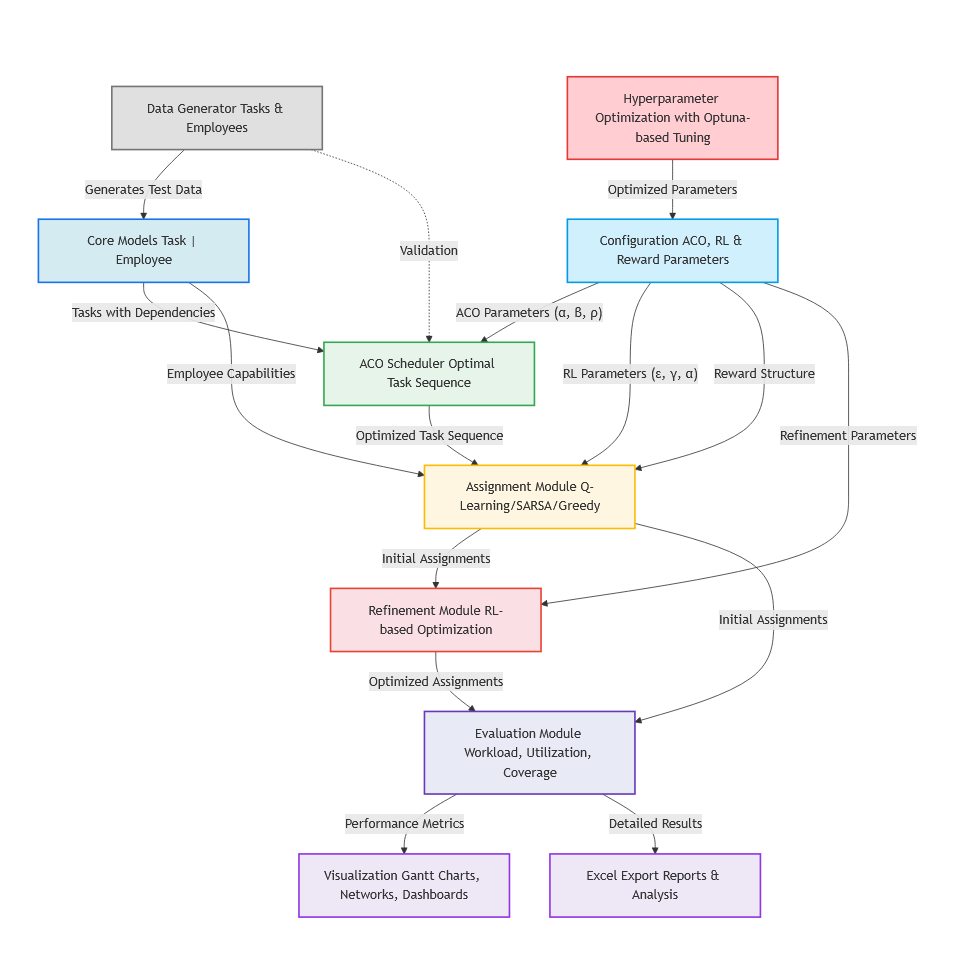
\includegraphics[width=1\linewidth]{figures/overall_architecture.png}
		\caption{\label{fig:arch}Architecture Diagram}
	\end{figure}
	
	\subsection{\label{subsec:framework}Framework Overview}
	
	The architecture is organized into three core modules:
	\begin{enumerate}
		\item \textbf{Task Sequencing:} An ACO-based module generates an initial task sequence by considering inter-task dependencies, deadlines, and priorities. The module leverages configurable parameters (e.g., pheromone influence $\alpha$, heuristic weight $\beta$, evaporation rate $\rho$, etc.) to guide the search.
		\item \textbf{RL-based Assignment:} Centralized RL agents (employing both Q-learning and SARSA variants) assign tasks to employees. The state representation includes the current task index, discretized measures of employee workload, and historical assignment data. An $\epsilon$-greedy policy—with optional Upper Confidence Bound (UCB) enhancements—is used to balance exploration and exploitation.
		\item \textbf{Post-Assignment Refinement:} A dedicated refinement module further optimizes the initial assignment. By iteratively adjusting the task-to-employee mapping based on updated workload distributions and unassigned tasks, this stage improves overall balance and skill alignment.
	\end{enumerate}
	
	\subsection{\label{subsec:task-seq}Task Sequencing via Ant Colony Optimization (ACO)}
	
	The ACO module starts by initializing a pheromone matrix $\mathbf{P}$ with parameters such as $\alpha$, $\beta$, and $\rho$ (all configurable via the system settings). Each task is assigned a heuristic value $\eta_{ij}$ based on factors like priority, estimated duration, and deadline constraints. The probability of transitioning from task $t_i$ to task $t_j$ is computed as:
	\begin{equation}
		p_{ij} = \frac{[\mathbf{P}_{ij}]^{\alpha} \,[\eta_{ij}]^{\beta}}{\sum_{k \in \mathcal{N}_i}[\mathbf{P}_{ik}]^{\alpha} \,[\eta_{ik}]^{\beta}}
	\end{equation}
	where $\mathcal{N}_i$ is the set of candidate tasks for task $t_i$. After constructing candidate sequences with multiple agents, the pheromone levels are updated by:
	\begin{equation}
		\mathbf{P}_{ij} \leftarrow (1 - \rho)\,\mathbf{P}_{ij} + \Delta \mathbf{P}_{ij}
	\end{equation}
	with $\Delta \mathbf{P}_{ij}$ reflecting the quality of the sequence. This process is re-invoked periodically (e.g., every few hundred training episodes) to adapt to evolving system conditions.
	
	\subsection{\label{subsec:rl-task}RL-based Task Assignment and Post-Assignment Refinement}
	
	The RL module formulates task assignment as a sequential decision process. The state $s$ captures the current task index, residual working hours for each employee, and a history of past assignments. Actions include assigning a task to an employee or opting to skip it if constraints cannot be met. For Q-learning, the update rule is:
	\begin{equation}
		Q(s,a) \leftarrow Q(s,a) + \alpha \left[r + \gamma \max_{a'} Q(s',a') - Q(s,a)\right]
	\end{equation}
	and for SARSA:
	\begin{equation}
		Q(s,a) \leftarrow Q(s,a) + \alpha \left[r + \gamma Q(s',a') - Q(s,a)\right]
	\end{equation}
	A scheduled decay of the exploration rate $\epsilon$, along with optional UCB adjustments, guides the learning process. Following the initial assignment, the \emph{RefinementRL} module further optimizes the allocation by considering an updated state $\mathcal{S}$ (comprising current workloads, the mapping of tasks to employees, and unassigned tasks) and applying a similar RL update:
	\begin{equation}
		Q(\mathcal{S},a) \leftarrow Q(\mathcal{S},a) + \alpha_r \left[r + \gamma_r \max_{a'} Q(\mathcal{S}',a') - Q(\mathcal{S},a)\right]
	\end{equation}
	Here, the refinement parameters $\alpha_r$ and $\gamma_r$ are tuned specifically to improve workload balance and alignment with employee skills.
	
	\begin{table}[!ht]
		\caption{\label{tab:legend}Legend of Symbols}
		\begin{ruledtabular}
			\begin{tabular}{ll}
				\textbf{Symbol}    & \textbf{Description}                                       \\
				\hline
				$i$                & Current task index                                         \\
				$\mathbf{P}$       & Pheromone matrix                                           \\
				$\eta_{ij}$        & Heuristic value for transitioning from task $t_i$ to $t_j$ \\
				$\rho$             & Pheromone evaporation rate                                 \\
				$s, s'$            & RL states before and after an action                       \\
				$a, a'$            & Actions chosen in the current and subsequent states        \\
				$\alpha, \alpha_r$ & Learning rates for initial assignment and refinement       \\
				$\gamma, \gamma_r$ & Discount factors for initial assignment and refinement     \\
				$\epsilon$         & Exploration rate in RL                                     \\
				$\mathbf{H}$       & Vector of residual working hours                           \\
				$r$                & Immediate reward signal                                    \\
				$\mathcal{S}$      & State representation for refinement                        \\
				$M$                & Task-to-employee mapping                                   \\
				$U$                & Set of unassigned tasks                                    \\
			\end{tabular}
		\end{ruledtabular}
	\end{table}
	
	
	\subsection{\label{subsec:hyperparameter}Hyperparameter Optimization and Experimental Evaluation}
	
	A standout feature of the design is the integration of automated hyperparameter tuning using Optuna. This module optimizes key parameters for both the ACO and RL components (such as learning rates, discount factors, exploration decay, and pheromone parameters) through a multi-objective process. The objectives are to maximize the proportion of tasks assigned and to minimize the variance of the reward signal. Extensive experimental trials yield Pareto-optimal configurations, with detailed visualizations and reports generated for comprehensive performance analysis.
	
	\section{\label{sec:inference}Inference and Discussion}
	Based on the simulation results we can notice that generated tasks are sorted by ACO step (\cref{fig:aco_sequence}) and also it combined with RL steps enhances the balance of task assignments among employees without compromising overall
	assignment rates or deadline compliance (\cref{fig:workload_balance_ratio,fig:greedy,fig:q_learning,fig:sarsa}).
	
	\subsection{\label{subsec:workload}Workload Distribution Insights}
	Results from the simulation (Fig.~\ref{fig:workload_balance_ratio}) indicate that greedy assignment methods typically overload a subset of employees due to repeated allocation of tasks that match their skill profiles. This concentration not only creates bottlenecks but also elevates the risk of fatigue and reduces overall efficiency. By integrating a workload balancing term into the reward function, the reinforcement learning module gradually redistributes tasks more evenly. As a result, the refined policies exhibit a substantial
	reduction in workload variance, as evidenced by a lower standard deviation of
	assigned hours relative to baseline approaches. This indicates that `RefinementRL` is working as intended. Notice how the Boring and Drilling tasks are handled in Greedy vs Refined Q-learning or SARSA  (\cref{fig:greedy,fig:q_learning,fig:sarsa}). Refined algorithms display better work balancing.
	
	\subsection{\label{subsec:rationale}Reward Dynamics}
	During both the initial and refinement stages, the reward structure used by the reinforcement learning components directly improved the workload balance. The reward functions penalized excessive task concentration instead of just encouraging rapid task completion tied to strict deadlines. Through multiple training episodes, the RL agents learned and internalized the cost of overburdening certain employees, which led to more even distribution of work and achieved the dual goals of efficiency and fairness in the scheduling process.
	
	The 70:30 epsilon decay schedule and the UCB mechanism complemented each other to improve reward performance. The UCB mechanism gave an exploration bonus to actions that were less visited, so that the agent would explore other actions before declaring an action optimal. The agents were able to learn better action value estimates earlier in this balanced exploration. In the meantime, the 70:30 decay schedule decreased the exploration rate during the first 70\% of the episodes (exploration vs exploitation) and kept a stable low exploration regime in the last 30\% of training. Together these strategies let the agents learn more robustly, with a steadily increasing moving average of rewards during training(\cref{fig:rewards_training}).
	
	\subsection{\label{subsec:tradeoffs}Practical Trade-offs and Future Considerations}
	Although the hybrid ACO-RL framework markedly improves workload distribution,
	its practical deployment requires careful tuning of reward parameters to align
	with organizational priorities. In certain scenarios, urgent tasks might
	necessitate a temporary deviation from perfect balance in order to assign
	critical tasks to the most qualified personnel. Future enhancements could include
	dynamic adjustment of reward components in response to real-time performance metrics.
	Overall, the incorporation of workload balance as a primary objective not only
	advances scheduling methodologies but also contributes to more resilient and sustainable
	workforce management.
	
	
	\subsection{\label{subsec:plots}Plots from the Simulation}
	
	\begin{figure}[H]
		\centering
		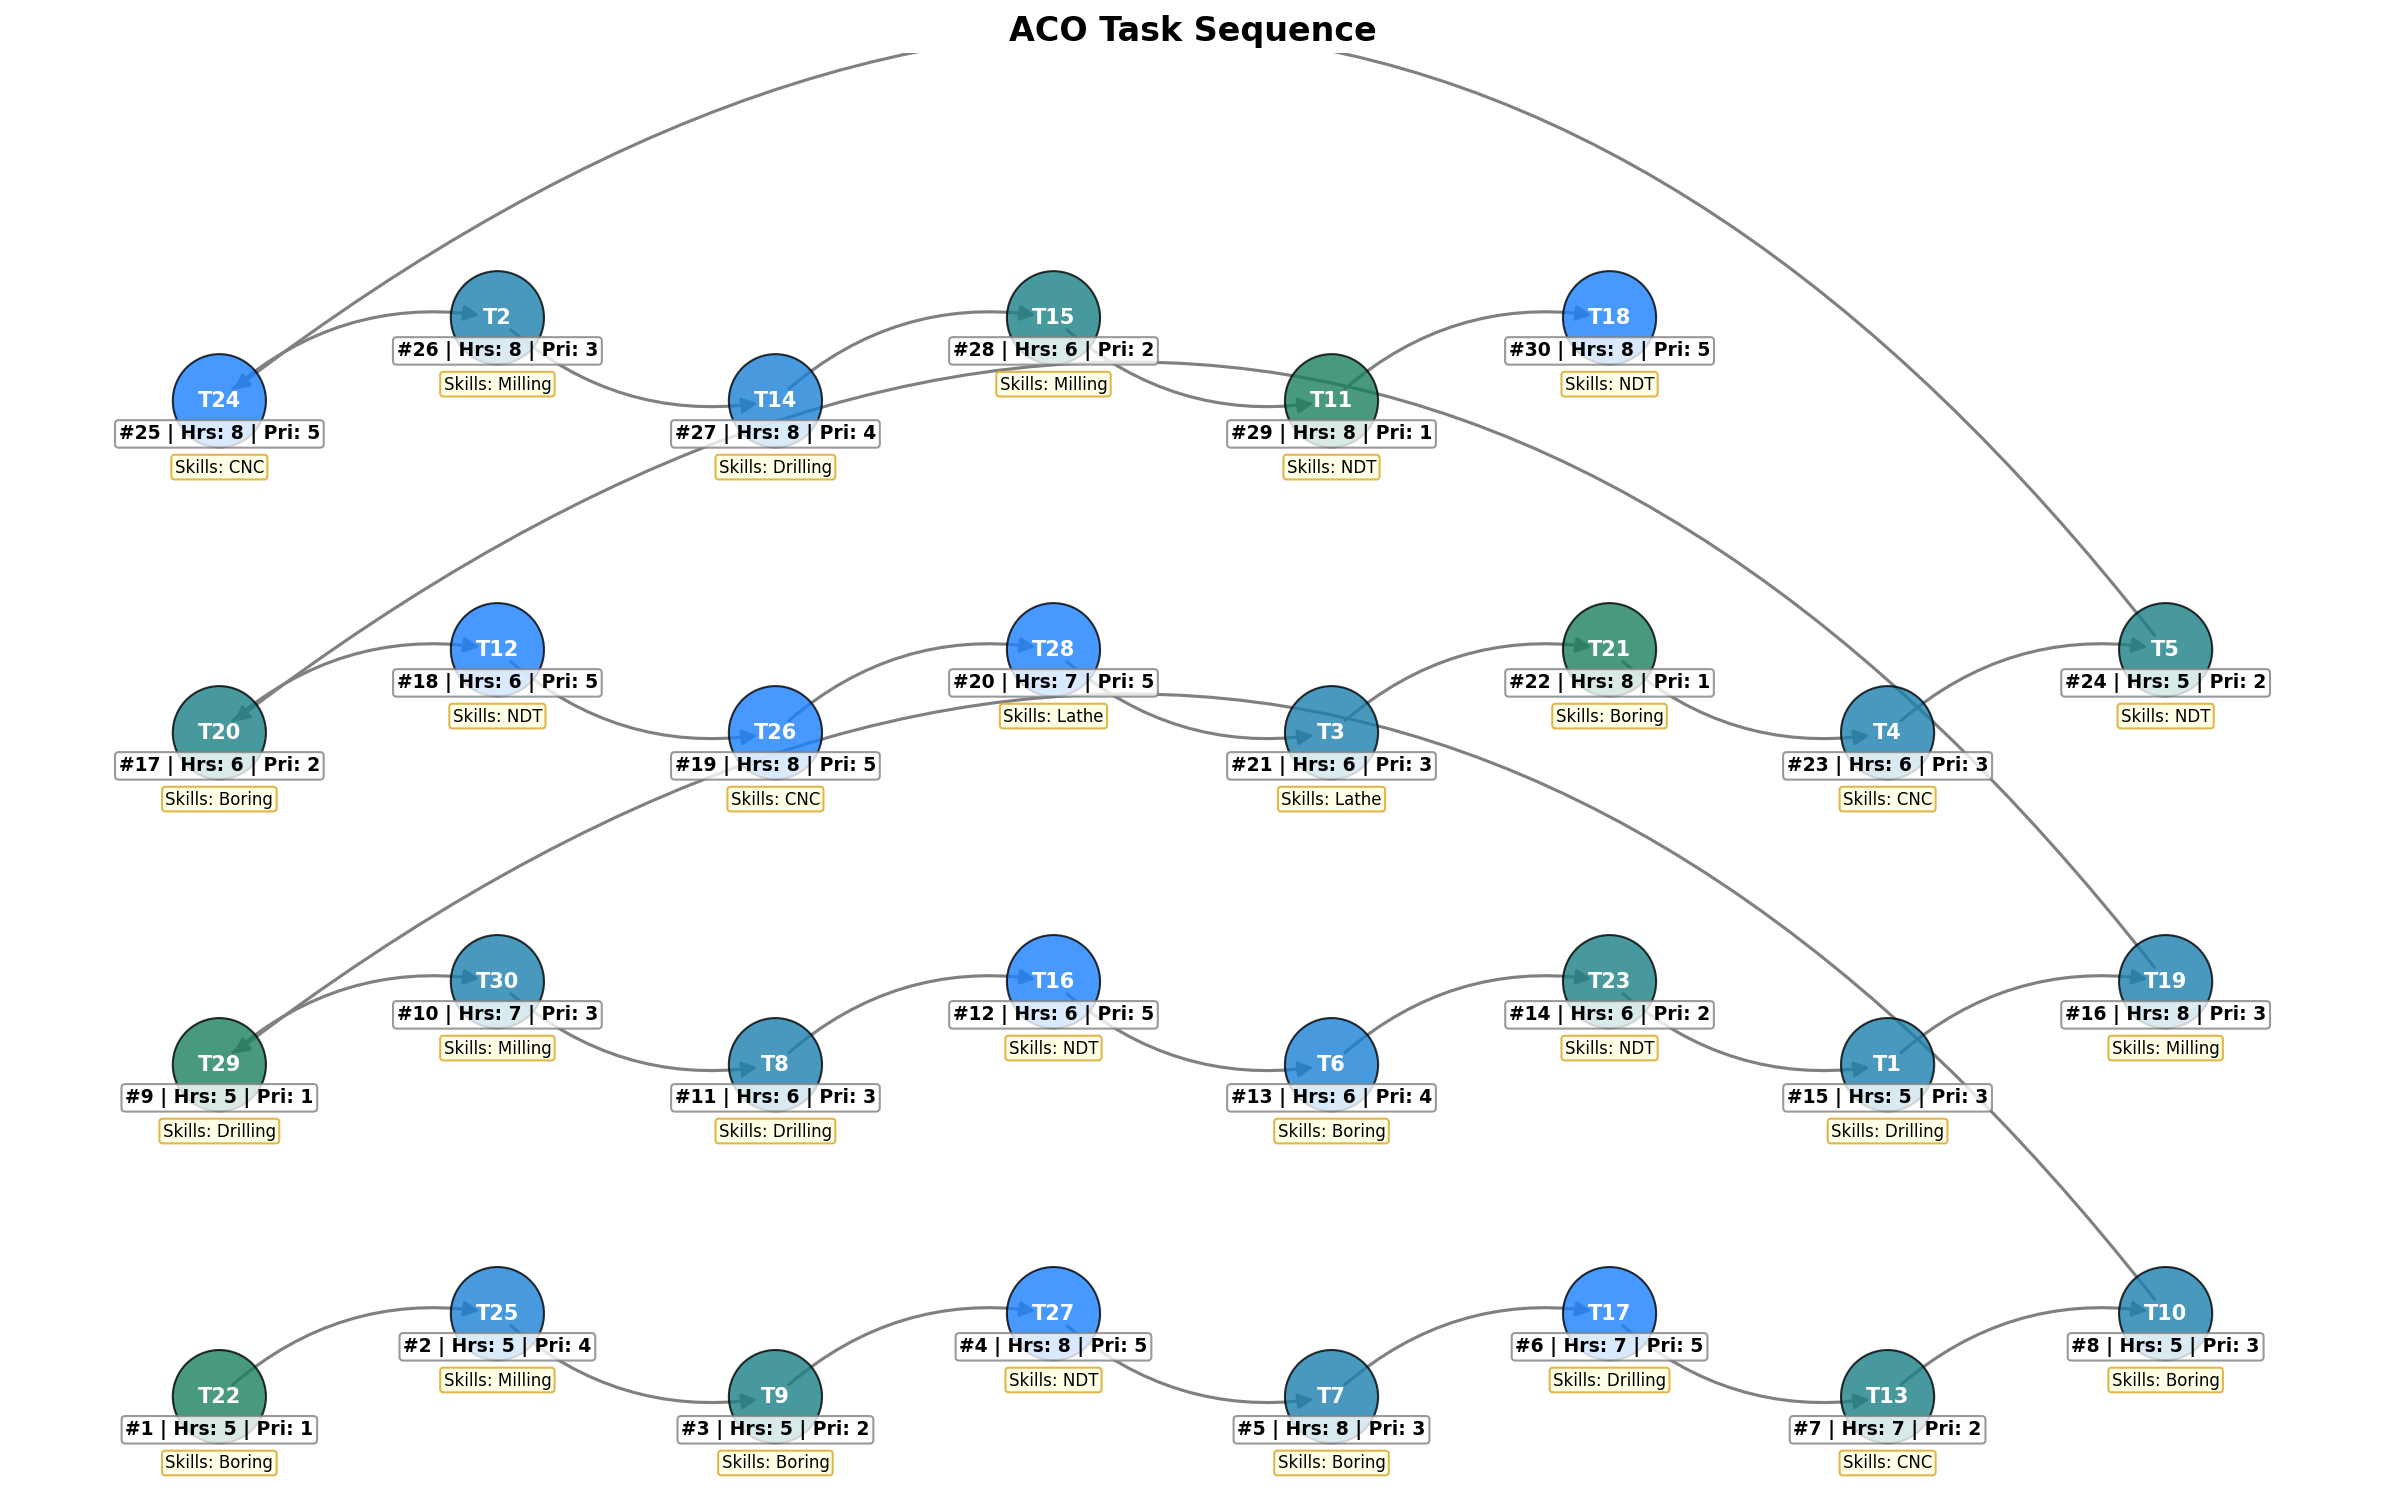
\includegraphics[width=1\textwidth]{figures/aco_network.png}
		\caption{\label{fig:aco_sequence}Illustration of the Ant Colony Optimization (ACO) task sequence.}
	\end{figure}
	
	\begin{figure}[H]
		\centering
		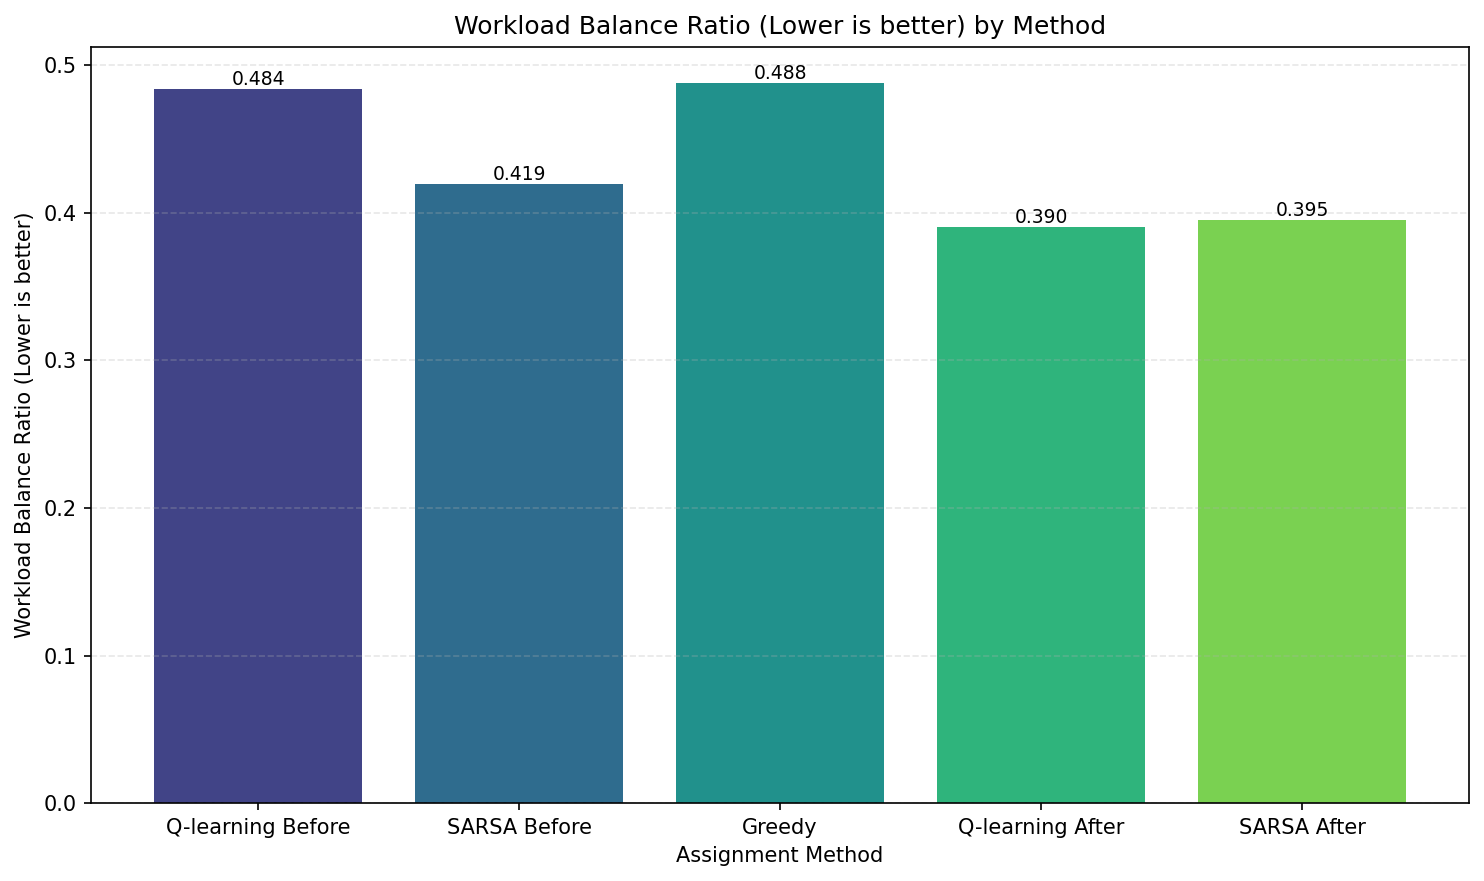
\includegraphics[width=1\textwidth]{figures/workload_balance_ratio_comparison.png}
		\caption{\label{fig:workload_balance_ratio}Workload Balance Ratio (lower is better) by assignment method.}
	\end{figure}
	
	\begin{figure}[H]
		\centering
		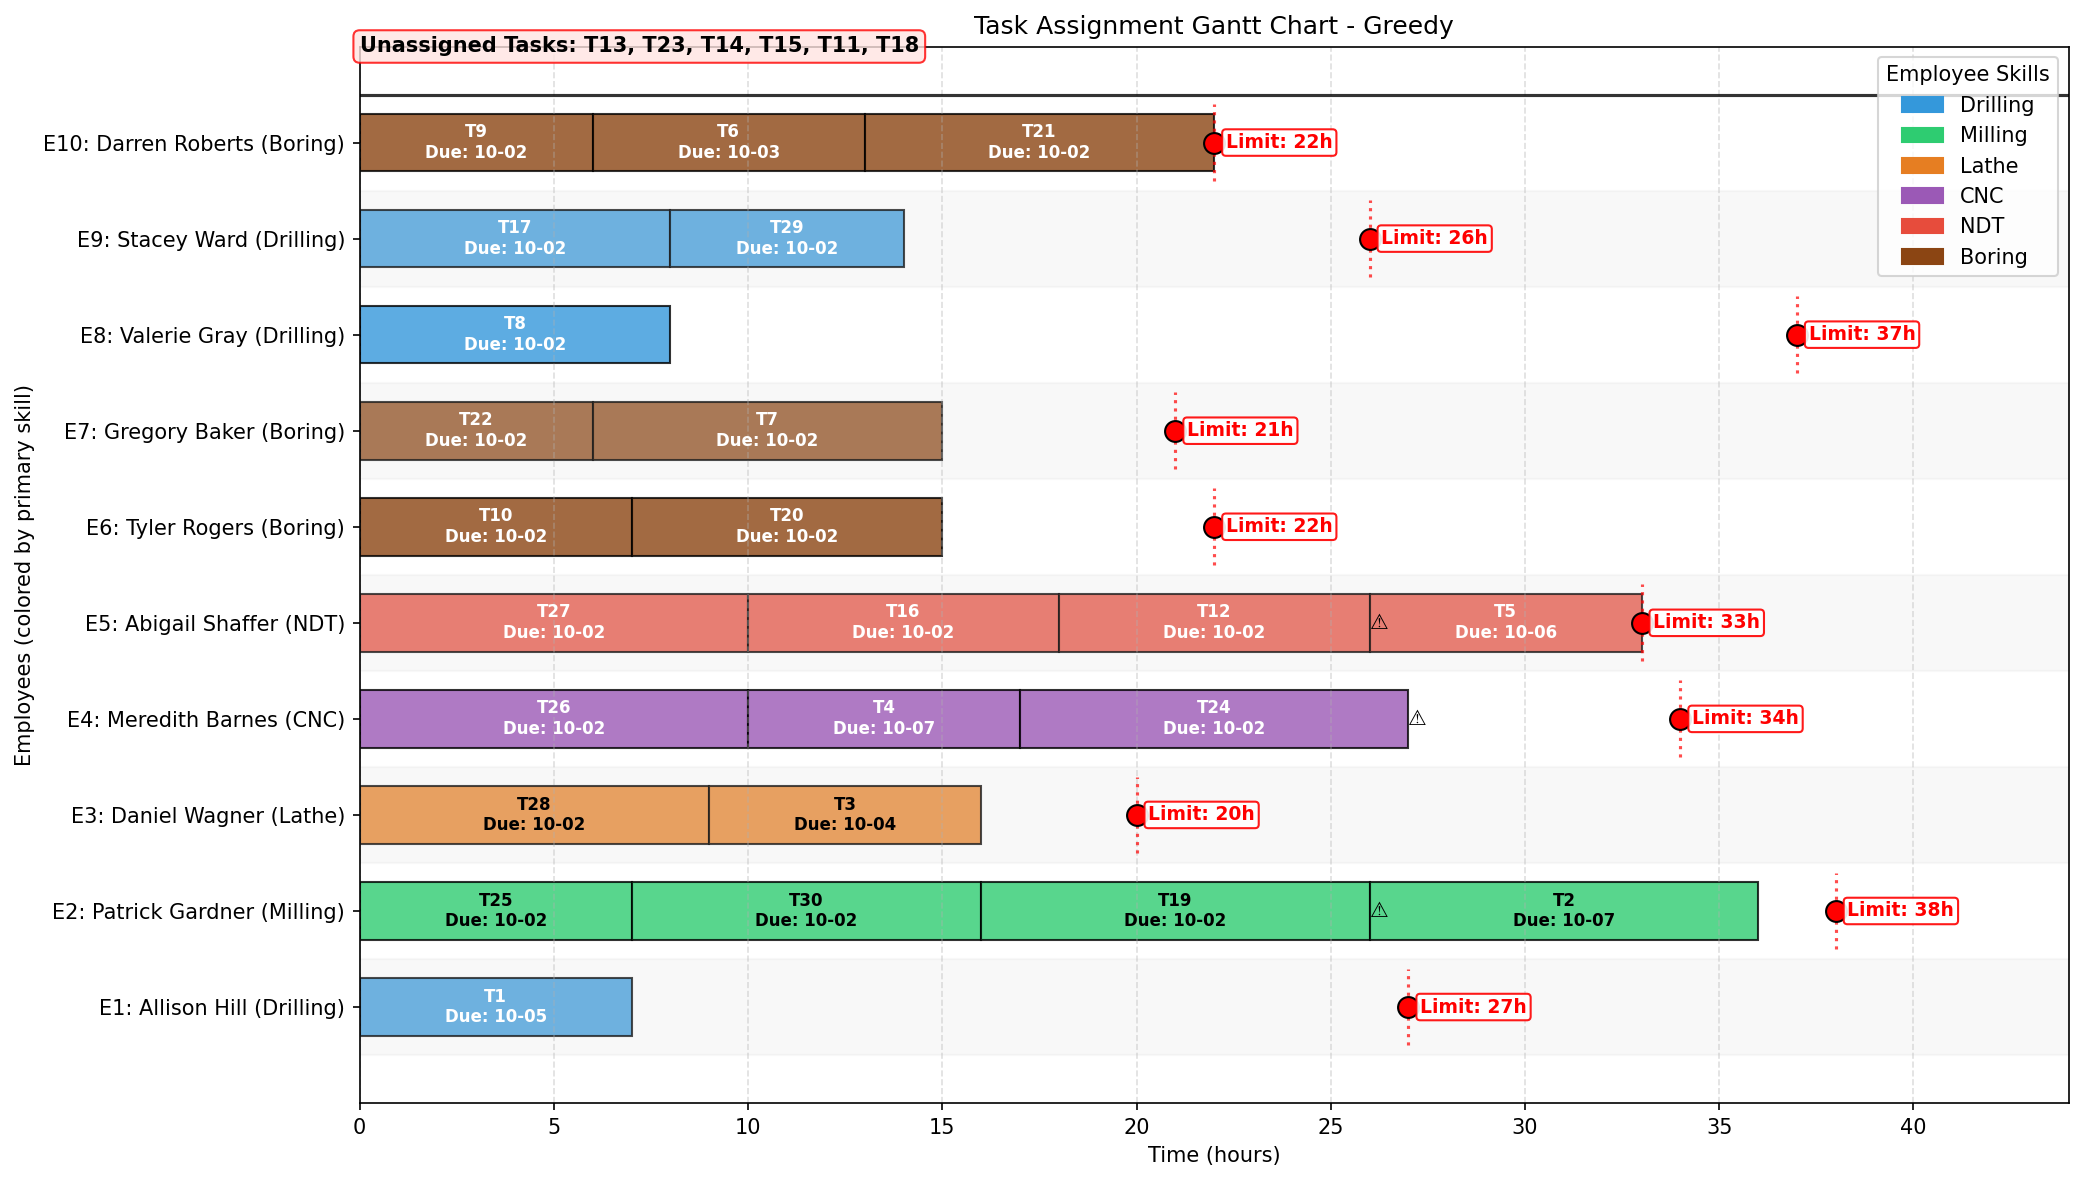
\includegraphics[width=1\textwidth]{figures/gantt_greedy.png}
		\caption{\label{fig:greedy}Assignments by Greedy method}
	\end{figure}
	
	\begin{figure}[H]
		\centering
		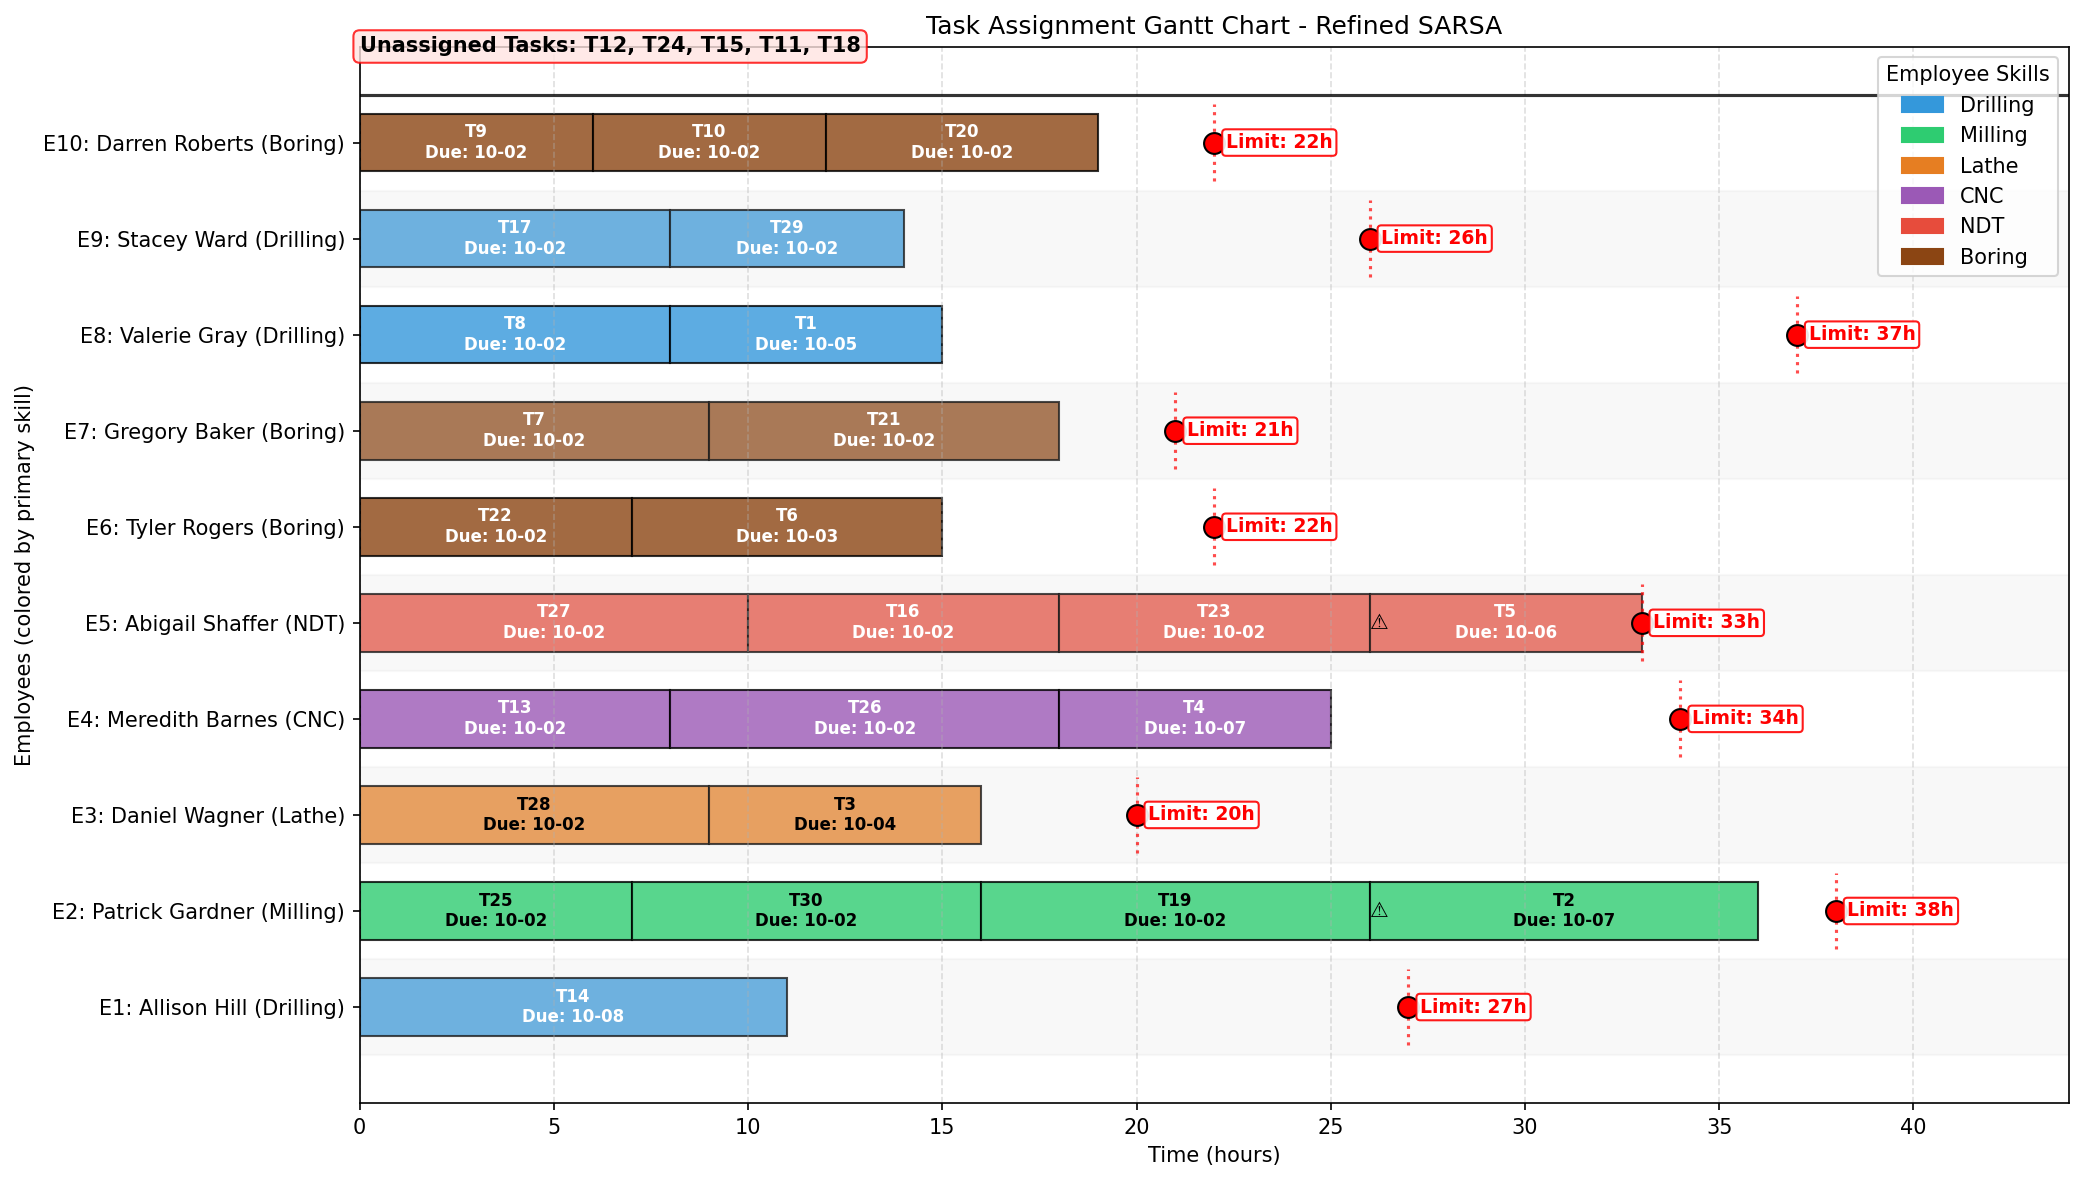
\includegraphics[width=1\textwidth]{figures/gantt_sarsa_after.png}
		\caption{\label{fig:sarsa}Assignments by SARSA after Refinement}
	\end{figure}
	
	\begin{figure}[H]
		\centering
		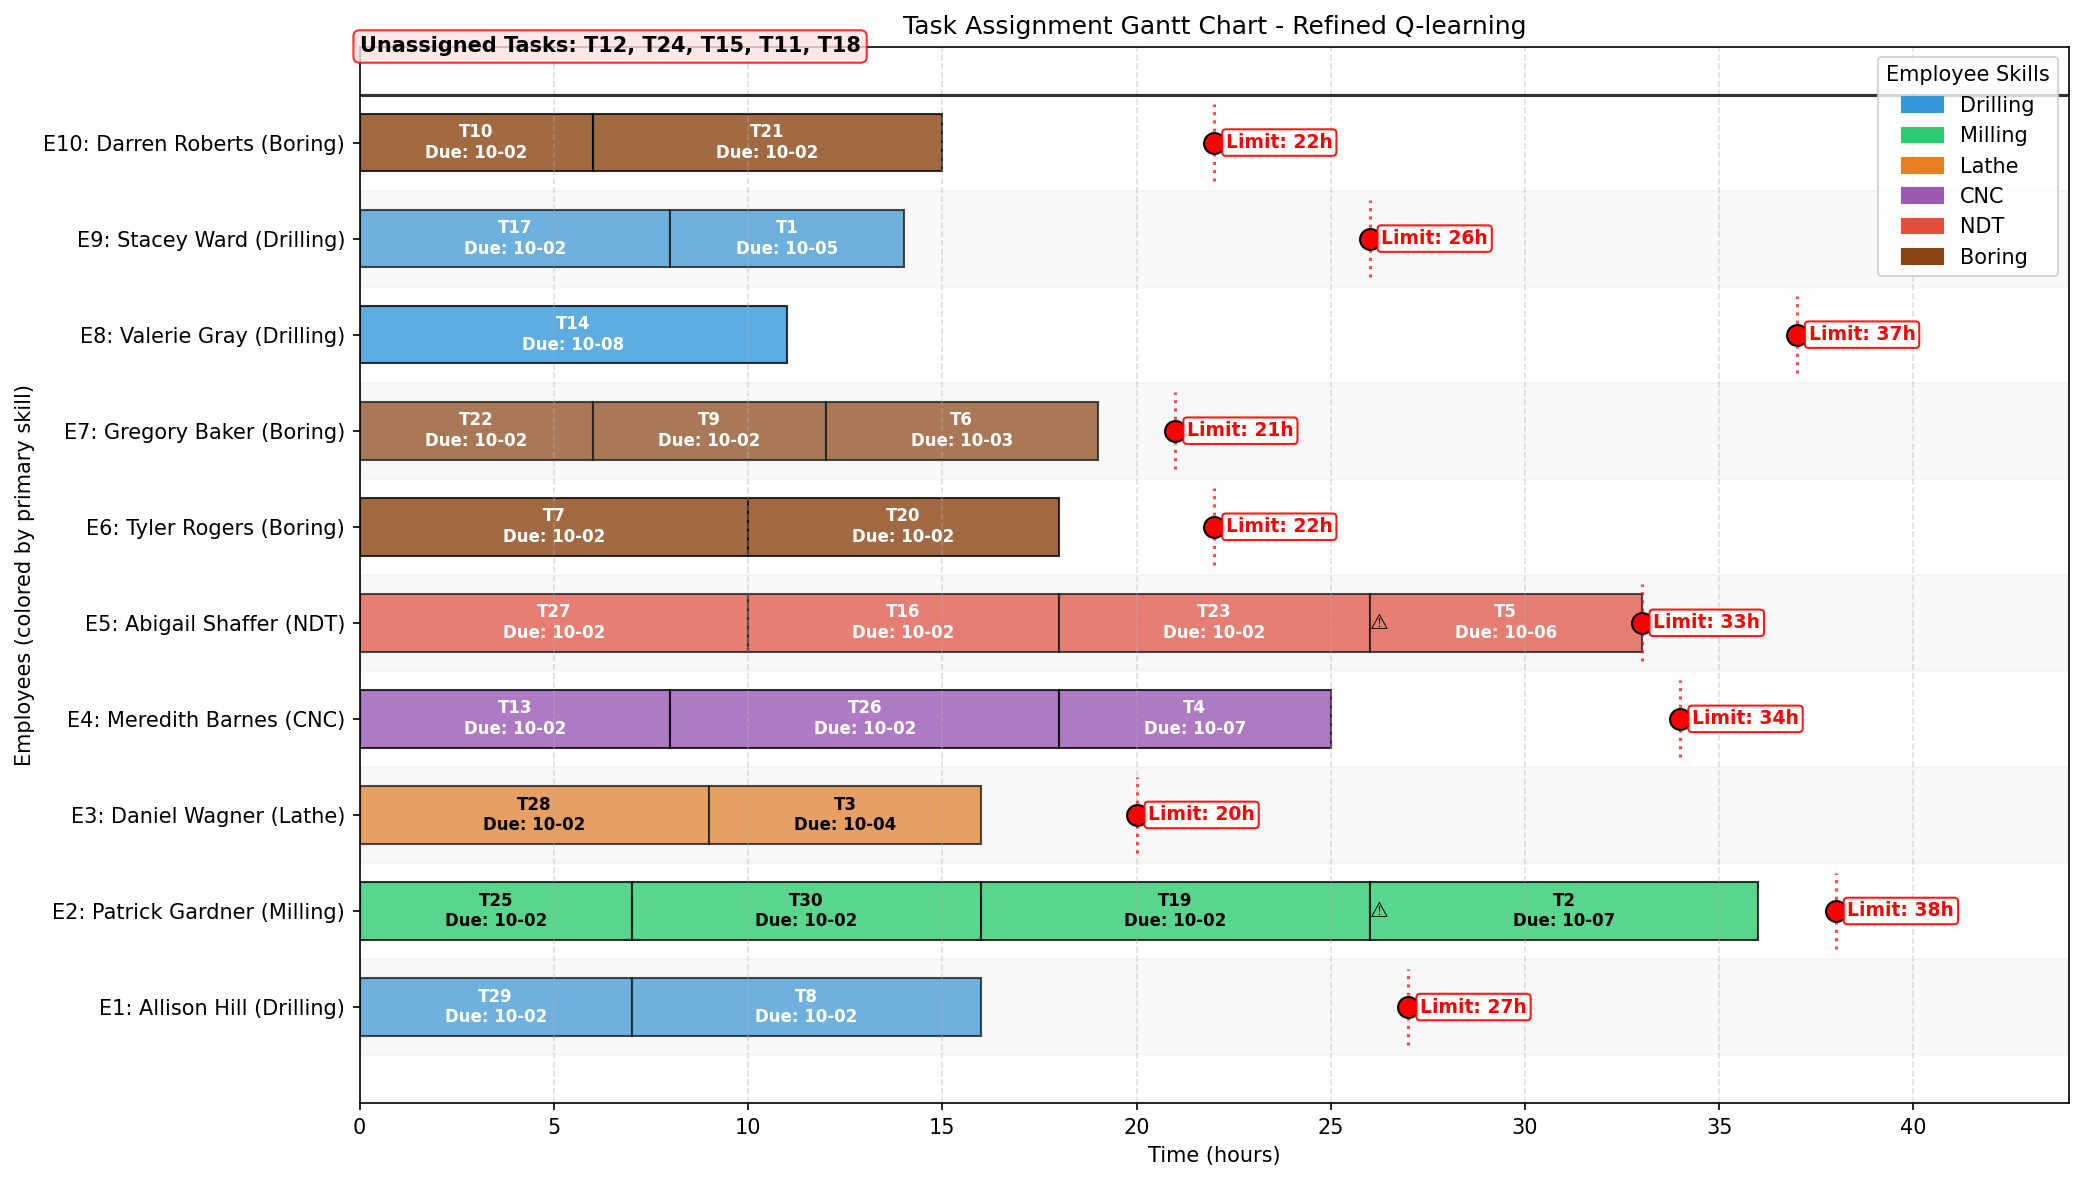
\includegraphics[width=1\textwidth]{figures/gantt_q_after.png}
		\caption{\label{fig:q_learning}Assignments by Q-learning after Refinement}
	\end{figure}
	
	\begin{figure}[H]
		\centering
		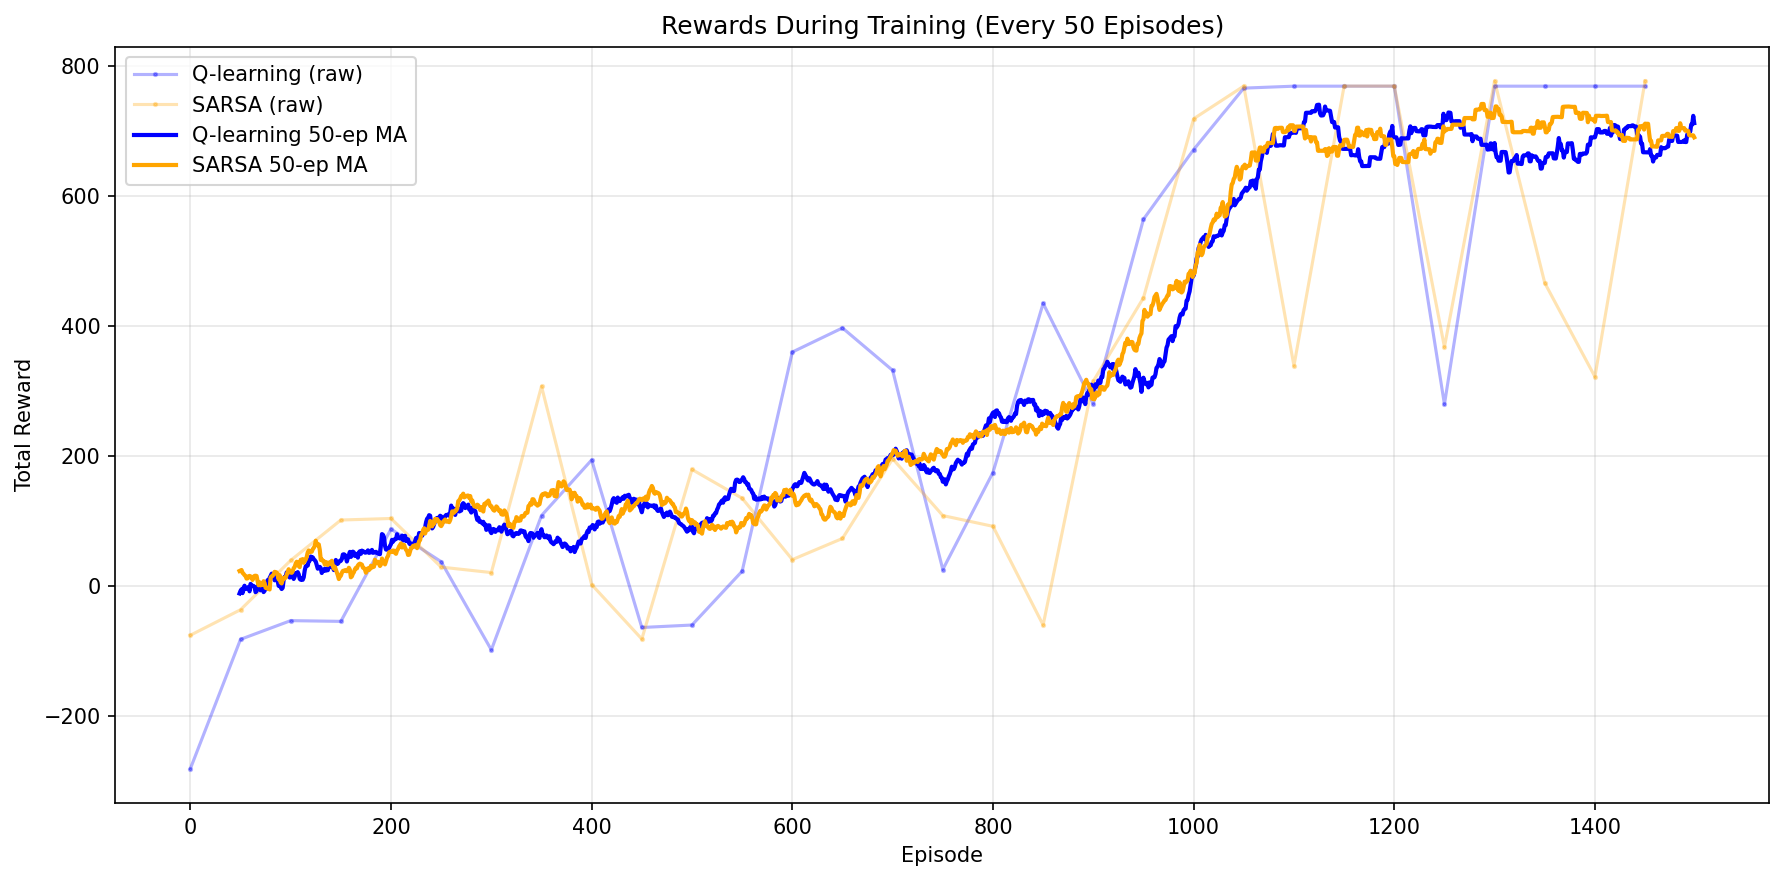
\includegraphics[width=1\textwidth]{figures/rewards_history.png}
		\caption{\label{fig:rewards_training}Rewards during training (with 50 MA).}
	\end{figure}
	
	\section{\label{sec:future}Future Work}
	
	While the current framework—which combines ACO-based task sequencing with
	reinforcement learning for employee assignment—has yielded promising results, several
	avenues for further research remain:
	
	\begin{itemize}
		\item \textbf{Enhanced State Representations:} The present RL models utilize
		discretized state representations. Future research could explore richer representations,
		such as deep neural network embeddings, to capture complex task dependencies
		and nuanced employee characteristics more effectively.
		
		\item \textbf{Hybrid Optimization Techniques:} Integrating additional
		meta-heuristic or evolutionary algorithms with ACO may lead to improved
		task sequencing. Investigating hybrid models that merge global search capabilities
		with localized refinement strategies could further optimize scheduling performance.
		
		\item \textbf{Adaptive Reward Mechanisms:} Given the critical role of the
		reward structure, future work could develop dynamic or adaptive reward schemes
		that adjust penalties and incentives based on real-time feedback or historical
		data, thereby enhancing both workload balance and resource utilization.
		
		\item \textbf{Scalability and Real-Time Implementation:} Although our
		experiments were conducted on a moderate scale, real-world applications often
		involve larger task sets and employee pools. Future studies should address
		scalability challenges and explore real-time implementations, possibly leveraging
		distributed computing frameworks.
		
		\item \textbf{Incorporating Uncertainty:} Extending the framework to account
		for uncertainties in task durations, employee availability, and
		environmental changes would increase its robustness. Incorporating probabilistic
		models or robust optimization techniques into the RL component may better handle
		stochastic variations.
		
		\item \textbf{User Feedback Integration:} Future systems could incorporate
		continuous feedback from domain experts and end-users, enabling a human-in-the-loop
		approach that iteratively refines both task sequencing and assignment processes
		based on practical, real-world insights.
	\end{itemize}
	
	These research directions aim to bridge the gap between theoretical scheduling
	models and practical, scalable solutions for dynamic, multi-agent systems. By addressing
	these challenges, future work can further enhance the adaptability and
	effectiveness of the hybrid framework in diverse industrial environments.
	
	\begin{acknowledgments}
		The authors would like to express their sincere gratitude to SRM Institute of
		Technology for providing the resources and support necessary for this study. We
		are especially grateful to Professor Dr. Krishnaraj N for his invaluable
		guidance, insightful suggestions, and continuous encouragement throughout the
		course of this study. His expertise and constructive feedback have been instrumental
		in shaping the direction and success of this work.
	\end{acknowledgments}
	
	
	\nocite{*}
	
	\begin{thebibliography}{99}

		
		\bibitem{SuttonBarto1998}
		R.~S. Sutton and A.~G. Barto, \emph{Reinforcement Learning: An Introduction}, MIT Press, 1998.
		
		\bibitem{li2024}
		J. Li, L. Zhang, Z. Li, and S. Zhang, ``Dynamic scheduling for flexible job shop based on MachineRank with deep reinforcement learning,'' \textit{Sci. Rep.}, vol. 14, no. 1, p. 12345, 2024. doi:10.1038/s41598-024-79593-8.
		
		\bibitem{zhang2022}
		M. Zhang, Y. Lu, Y. Hu, N. Amaitik, and Y. Xu, ``Dynamic Scheduling Method for Job-Shop Manufacturing Systems by Deep Reinforcement Learning with Proximal Policy Optimization,'' \textit{Sustainability}, vol. 14, no. 9, p. 5177, 2022. doi:10.3390/su14095177.
		
		
		
		\bibitem{wang2023}
		Wang B, Liu Y, Qian J, Parker SK. The remote revolution: assessing the impact of working from home on employees' productivity and work-life balance. \textit{Future Business Journal}. 2023;9(1):1-14. doi:10.1186/s43093-024-00345-1.
		
		\bibitem{infantes2024} G. Infantes et al., ``Learning to Solve Job Shop Scheduling
		under Uncertainty,'' CPAIOR, 2024.
		
		\bibitem{burdett2004} R. L. Burdett and E. Kozan, ``The Assignment of
		Individual Renewable Resources in Scheduling,'' Asia Pacific Journal of
		Operational Research, 2004.
		
		\bibitem{zhong2024} L. Zhong, ``Comparison of Q-learning and SARSA
		Reinforcement Learning Models on Cliff Walking Problem,'' DAI, 2024.
		
		\bibitem{noureddine2017} D. Ben Noureddine et al., ``Multi-agent Deep Reinforcement
		Learning for Task Allocation in Dynamic Environment,'' ICSOFT, 2017.
		
		\bibitem{joo2022} T. Joo et al., ``Task Allocation in Human–Machine Manufacturing
		Systems Using Deep Reinforcement Learning,'' Sustainability, 2022.
		
		\bibitem{wibisono2016} A. Wibisono, A. S. Nisafani, H. Bae, and Y. Park, ``A dynamic
		and human-centric resource allocation for managing business process execution,''
		University of Texas at El Paso, Tech. Rep., Dec. 2016.
		
		\bibitem{dastmalchian2001} A. Dastmalchian and P. Blyton, ``Workplace flexibility
		and the changing nature of work: An introduction,'' \textit{J. Management Studies},
		vol. 38, no. 2, pp. 281-286, 2001.
		
		\bibitem{dorigo2016} M. Dorigo and T. Stützle, ``Ant colony optimization:
		Overview and recent advances,'' in \textit{Handbook of Metaheuristics}, 3rd
		ed. Springer, 2016, pp. 311-351.
		
		\bibitem{turn0file0} S. Ramesh, S. B. N., S. J. Sathyavarapu, V. Sharma, N. K. A. A., and M. Khanna, ``Comparative analysis of Q-learning, SARSA, and deep Q-network for microgrid energy management,'' \textit{Scientific Reports}, vol. 15, p. 694, 2025, doi:10.1038/s41598-024-83625-8.
		
		\bibitem{turn0file1} K. Sivamayil, E. Rajasekar, B. Aljafari, S. Nikolovski, S. Vairavasundaram, and I. Vairavasundaram, ``A systematic study on reinforcement learning based applications,'' \textit{Energies}, vol. 16, p. 1512, 2023, doi:10.3390/en16031512.
		
		\bibitem{Corazza2015} 
		M. Corazza and A. Sangalli, ``Q-Learning and SARSA: A Comparison between Two Intelligent Stochastic Control Approaches for Financial Trading,'' Working Paper, Ca’ Foscari University of Venice, 2015. Available: \url{https://ssrn.com/abstract=2617630}.
		
		\bibitem{Mavrovouniotis2023} 
		M. Mavrovouniotis, M. N. Anastasiadou, and D. Hadjimitsis, ``Measuring the Performance of Ant Colony Optimization Algorithms for the Dynamic Traveling Salesman Problem,'' \textit{Algorithms}, vol. 16, no. 545, 2023, doi: 10.3390/a16120545. Available: \url{https://doi.org/10.3390/a16120545}.
		
		\bibitem{Akiba2019Optuna} 
		T. Akiba, S. Sano, T. Yanase, T. Ohta, and M. Koyama, \emph{Optuna: A Next-generation Hyperparameter Optimization Framework}, Preprint, compiled July 26, 2019.
		
		
		\bibitem{Wang2023TaskScheduling} 
		Y. Wang, S. Dong, and W. Fan, \emph{Task Scheduling Mechanism Based on Reinforcement Learning in Cloud Computing}, Mathematics, vol. 11, 3364, 2023, doi:10.3390/math11153364.
		
	\end{thebibliography}
	
	\section{\label{sec:appendix}Appendix}
	The source code for this project is available on GitHub at \url{https://github.com/samkrdev/Hybrid-ACO-RL-Task-assigner}.
	
	
	
\end{document}